\documentclass[11pt,a4paper]{article}
\usepackage[T1]{fontenc}
\usepackage{lmodern}
\usepackage[slovene]{babel}
\usepackage[margin=2.5cm]{geometry}
\usepackage{graphicx} % Required for inserting images
\usepackage{url} % za povezave v virih
\usepackage{array} % poravnava besedila v tabeli

\title{Pregled obstoječih rešitev\\[4pt] \large Projekt: spletna stran podjetja MB Tech}
\author{Luka Petrović \and Matic Bas \and Matic Peterlin}
\date{23. november 2026}

\begin{document}

\maketitle

\tableofcontents

\section{Uvod}

\emph{MB Tech} je trgovina z računalniško opremo in servis iz Maribora. Podjetje prodaja
prenosnike, računalnike, telefone in dodatno opremo, popravlja naprave, sestavlja
računalnike po meri in svetuje pri nakupu študentom in podjetjem. V okviru projekta
izdelujemo spletno stran tega podjetja.

\textbf{Problem, ki ga rešujemo:} kupec, ki potrebuje novo opremo in hkrati popravilo
obstoječe naprave, mora danes pogosto uporabljati več različnih ponudnikov: velike
spletne trgovine za nakup in ločen servis za popravila. Okvirne cene popravil pogosto
niso objavljene, o stanju popravila pa stranka običajno izve šele po telefonu. Naša
spletna stran bo kupcem iz Maribora in okolice na enem mestu omogočila:

\begin{itemize}
\item pregled in iskanje izdelkov,
\item spletno naročilo servisa,
\item vpogled v cenik storitev,
\item sledenje stanju popravila.
\end{itemize}

Pred razvojem smo pregledali tri obstoječe slovenske rešitve, ki so podobne našemu
projektu: spletno trgovino \textbf{Big Bang}, spletno trgovino \textbf{Mimovrste} in
specializirano računalniško trgovino \textbf{Komponentko} (razdelek \ref{pregled}).
Primerjavo povzema tabela \ref{tabela1}, v razdelku \ref{zakljucek} pa opišemo, kaj
bomo prevzeli in kaj bo naša rešitev naredila drugače.

\section{Pregled obstoječih rešitev}
\label{pregled}

\subsection{Big Bang}

Big Bang je slovenski trgovec z avdio-video opremo in računalništvom s prodajnimi
mesti po vsej Sloveniji, med drugim tudi v Mariboru \cite{bigbang-ceneje}. Na spletni
strani navaja 14 prevzemnih mest \cite{bigbang}, v spletni trgovini pa ponuja več kot
15.000 izdelkov iz vseh oddelkov \cite{bigbang-ceneje}. Domača stran je prikazana na
sliki \ref{slika1}.

% slika Big Bang
\begin{figure}[h]
\centering
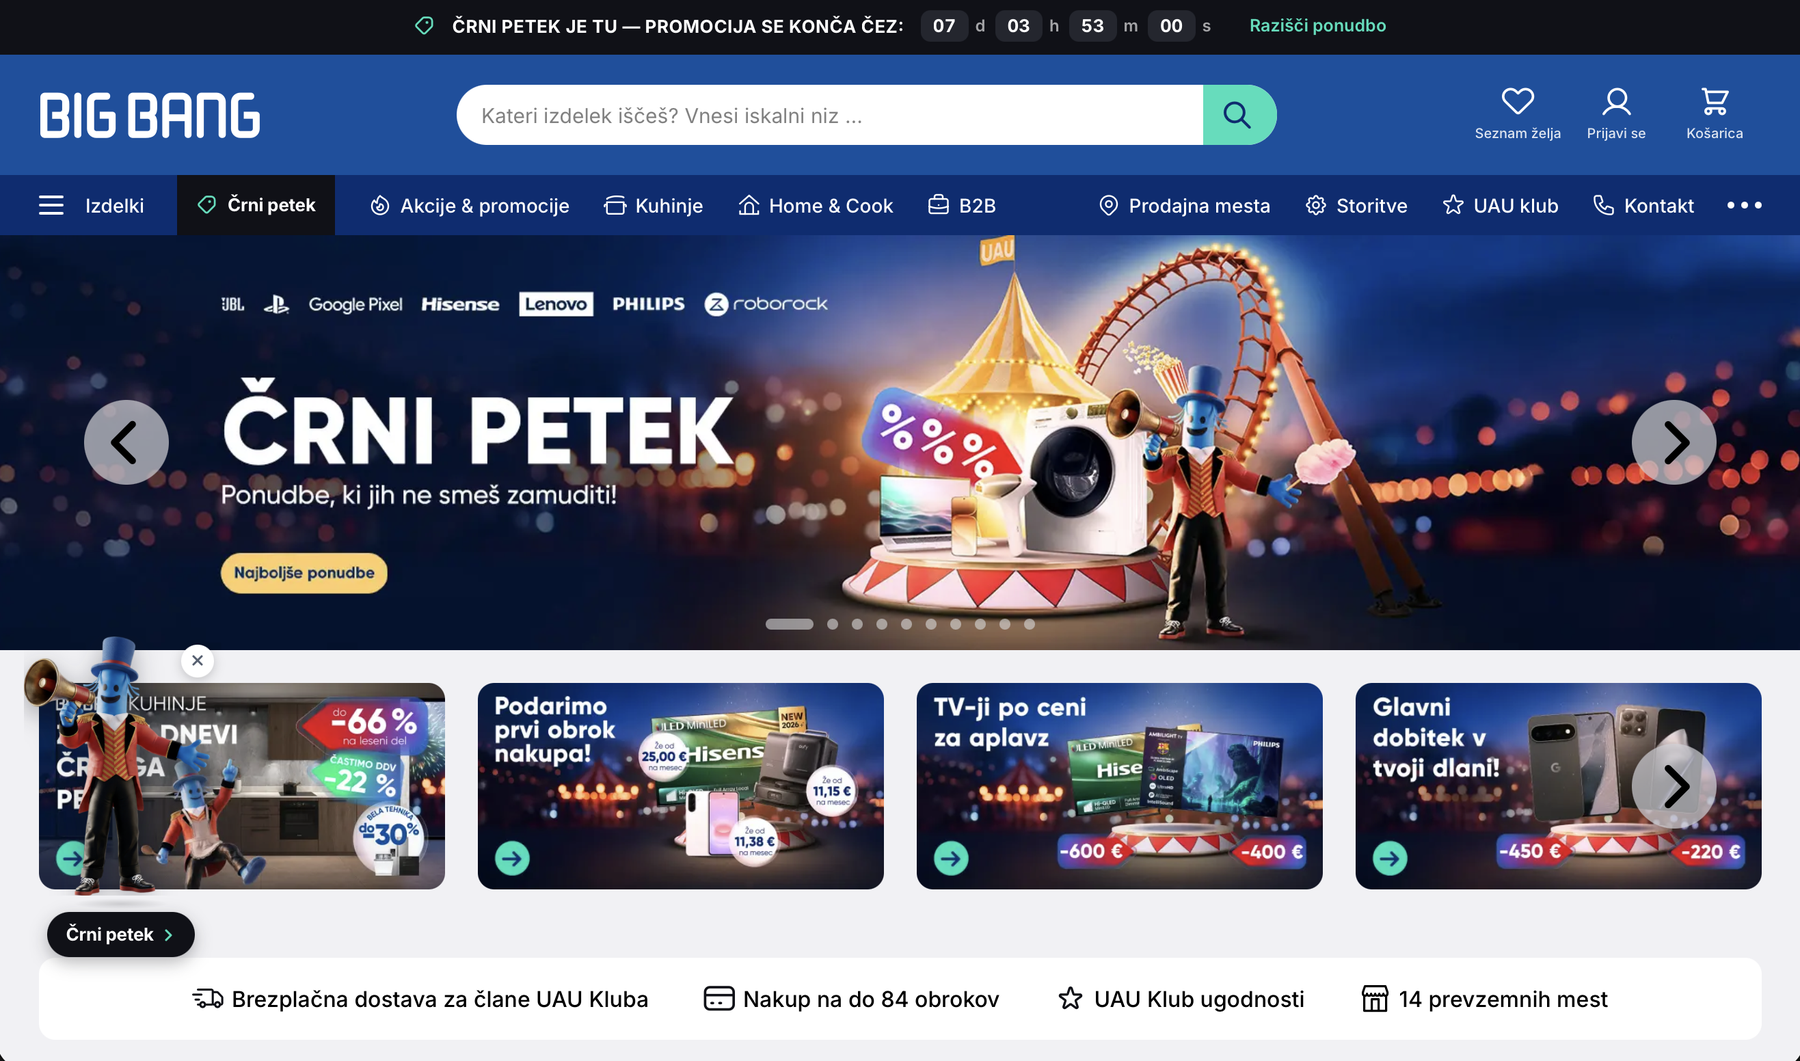
\includegraphics[width=\textwidth]{bigbang.png}
\caption{Domača stran spletne trgovine Big Bang \cite{bigbang}.}
\label{slika1}
\end{figure}

\textbf{Ključne funkcionalnosti:}
\begin{itemize}
\item glava strani z iskalnikom, seznamom želja, prijavo in košarico \cite{bigbang},
\item glavni meni s povezavami do izdelkov, akcij, prodajnih mest, storitev in kontakta \cite{bigbang},
\item klub zvestobe UAU z ugodnostmi, med drugim z brezplačno dostavo za člane \cite{bigbang},
\item nakup na do 84 obrokov \cite{bigbang} in drugi načini plačila (kartica, UPN, predračun, kredit) \cite{bigbang-ceneje},
\item prevzem v poslovalnici ali dostava po pošti, za večje izdelke tudi dostava z vnosom novega in odvozom starega aparata \cite{bigbang-ceneje}.
\end{itemize}

\textbf{Prednosti:}
\begin{itemize}
\item zelo velika izbira izdelkov na enem mestu,
\item prodajna in prevzemna mesta po vsej Sloveniji, tudi v Mariboru,
\item brezplačna dostava po pošti za naročila do 5~kg v vrednosti vsaj 99,99~€ \cite{bigbang-ceneje}.
\end{itemize}

\textbf{Slabosti:}
\begin{itemize}
\item računalniška oprema je le eden izmed mnogih oddelkov, zato svetovanje ni tako osebno kot v specializirani trgovini,
\item domača stran je polna oglasnih pasic in akcij, zato je manj pregledna,
\item stran je usmerjena v prodajo, ne v popravila računalnikov,
\item nekateri kupci pogrešajo plačilo s PayPalom \cite{bigbang-mnenja}.
\end{itemize}

\subsection{Mimovrste}

Mimovrste je slovenska spletna trgovina, ki deluje od leta 2002 \cite{mimovrste-ceneje}
in se predstavlja kot največja spletna trgovina v Sloveniji \cite{mimovrste-zaposlitev}.
Ponuja več kot dva milijona artiklov v 17 oddelkih \cite{mimovrste-ceneje}, danes pa je
del skupine Allegro \cite{mimovrste-allegro}. Domača stran je prikazana na sliki
\ref{slika2}.

% slika Mimovrste
\begin{figure}[h]
\centering
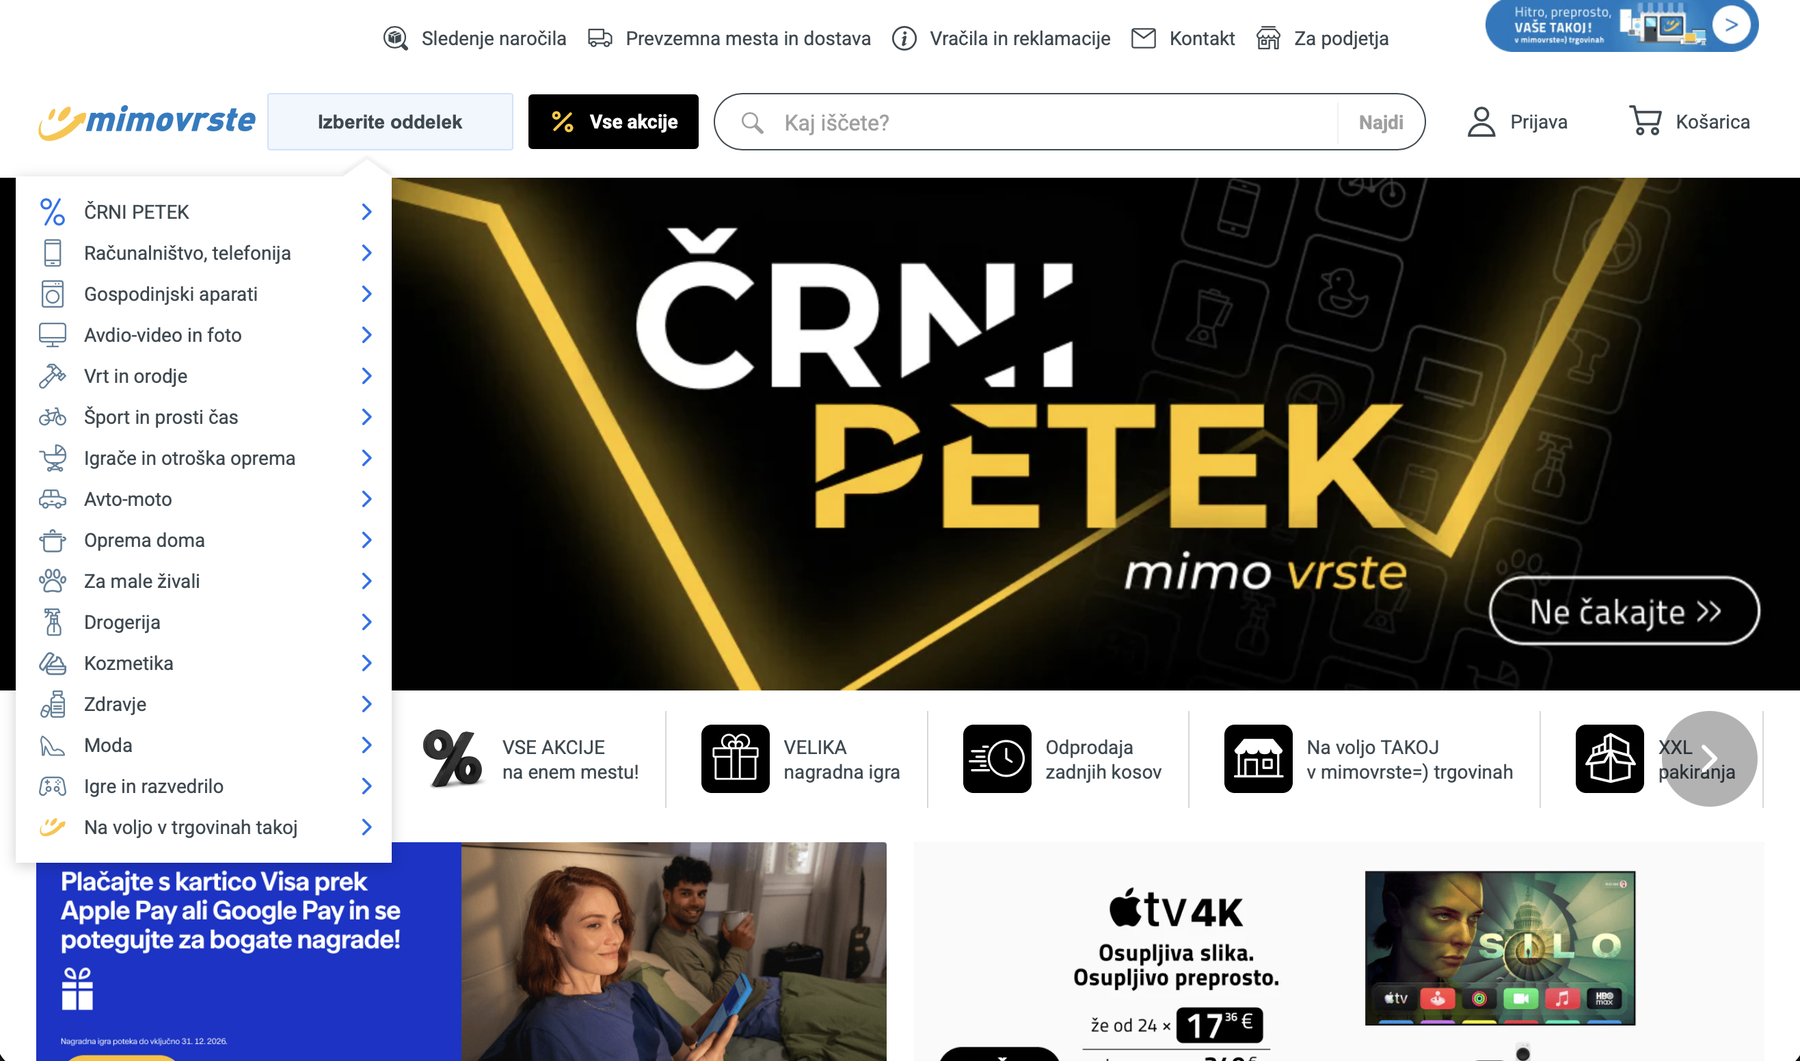
\includegraphics[width=\textwidth]{mimovrste.png}
\caption{Domača stran spletne trgovine Mimovrste \cite{mimovrste}.}
\label{slika2}
\end{figure}

\textbf{Ključne funkcionalnosti:}
\begin{itemize}
\item iskalnik, izbira oddelka, razdelek z vsemi akcijami, prijava in košarica \cite{mimovrste},
\item sledenje naročila, informacije o prevzemnih mestih in dostavi, vračila in reklamacije \cite{mimovrste},
\item mobilna aplikacija za nakupovanje \cite{mimovrste-app},
\item prevzemna mesta po Sloveniji, tudi v Mariboru \cite{mimovrste-enote}, in fizične trgovine \cite{mimovrste-trgovina},
\item plačilo z gotovino ob prevzemu, z nakazilom ali s kartico \cite{mimovrste-ceneje}.
\end{itemize}

\textbf{Prednosti:}
\begin{itemize}
\item ogromna izbira izdelkov iz zelo različnih področij,
\item nakupovanje tudi prek mobilne aplikacije,
\item kupec lahko sam spremlja, kje je njegovo naročilo,
\item prevzemno mesto v Mariboru.
\end{itemize}

\textbf{Slabosti:}
\begin{itemize}
\item splošna trgovina, ki ni specializirana za računalniško opremo,
\item veliko oglasnih pasic na domači strani odvrača pozornost od iskanja,
\item stran je namenjena prodaji in ne ponuja naročila popravila ali osebnega svetovanja.
\end{itemize}

\subsection{Komponentko}

Komponentko je specializirana slovenska računalniška trgovina, ki prodaja novo in
preverjeno rabljeno računalniško opremo \cite{komponentko-ceneje}. Poslovalnica je v
Ljubljani \cite{komponentko-ceneje}. Od pregledanih rešitev je najbolj podobna našemu
projektu, saj \underline{združuje trgovino in servis}. Domača stran je prikazana na
sliki \ref{slika3}.

% slika Komponentko
\begin{figure}[h]
\centering
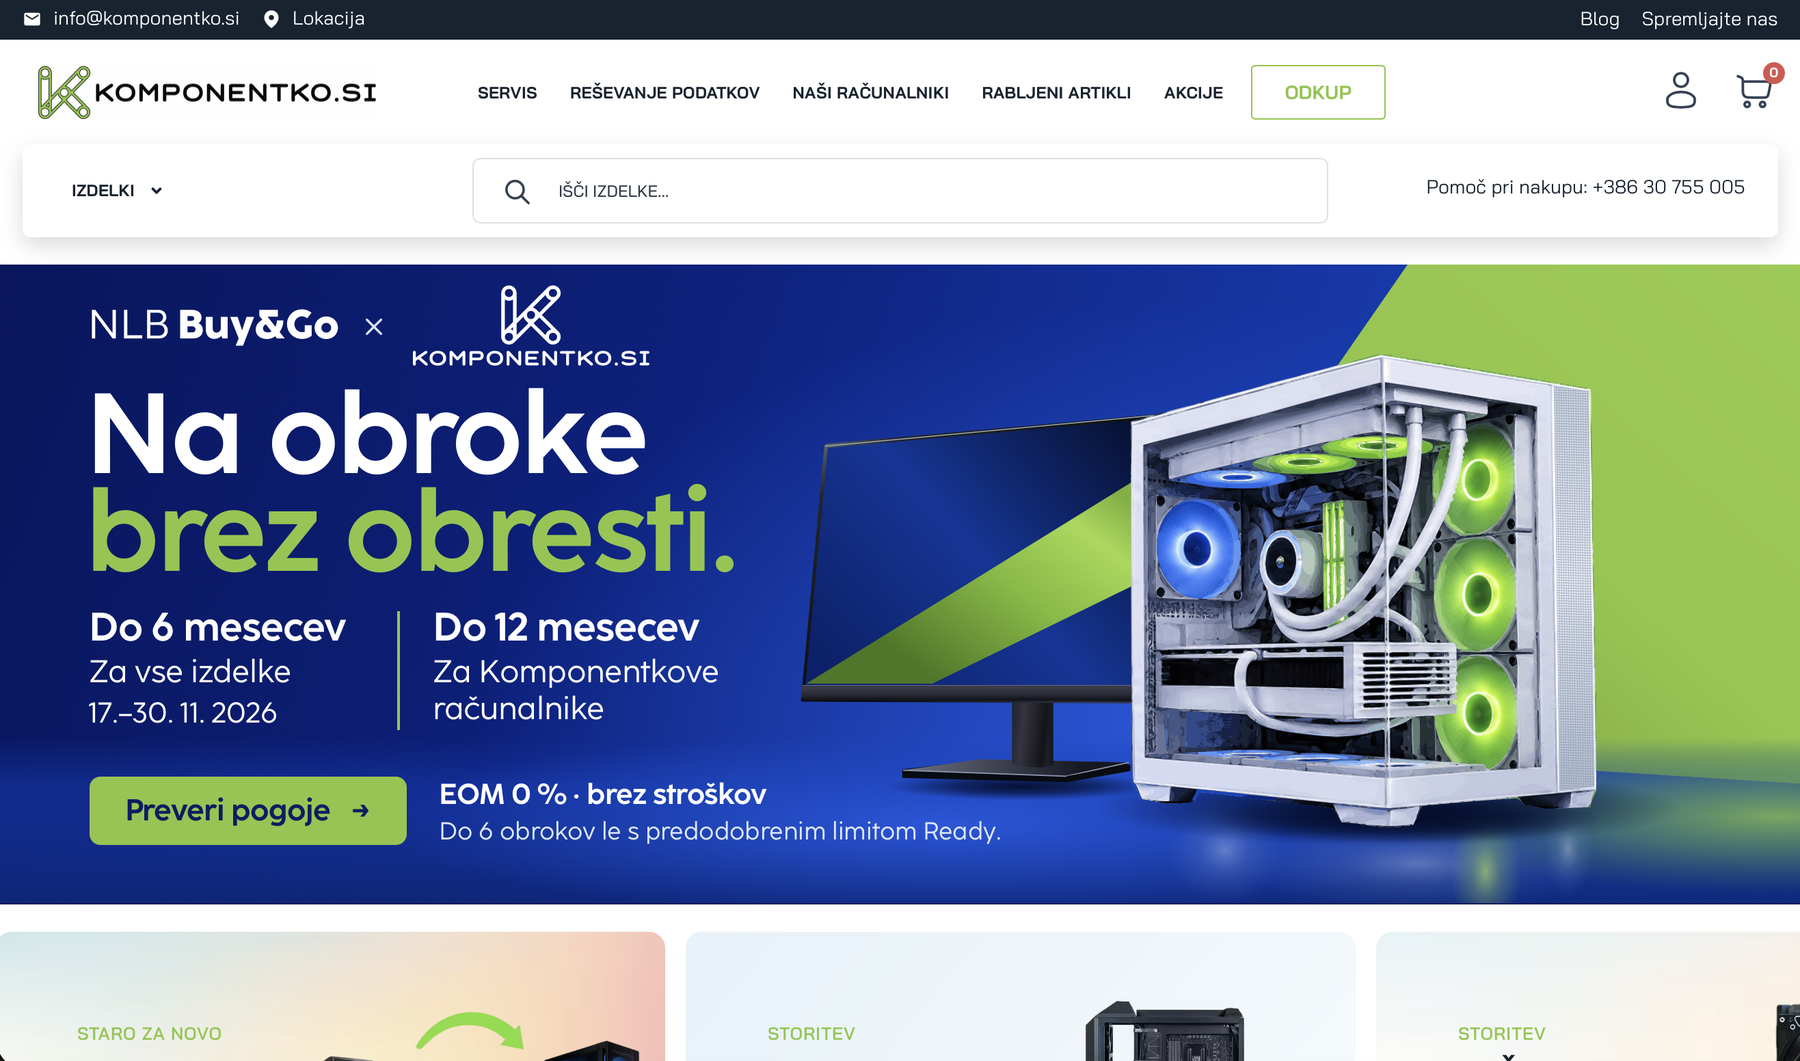
\includegraphics[width=\textwidth]{komponentko.png}
\caption{Domača stran računalniške trgovine Komponentko \cite{komponentko}.}
\label{slika3}
\end{figure}

\textbf{Ključne funkcionalnosti:}
\begin{itemize}
\item glavni meni s povezavami Servis, Reševanje podatkov, Naši računalniki, Rabljeni artikli, Akcije in Odkup \cite{komponentko},
\item iskalnik, meni izdelkov in telefonska številka za pomoč pri nakupu \cite{komponentko},
\item lasten servis, ki diagnostiko in popravila pogosto opravi v 48 urah, ter reševanje podatkov \cite{komponentko-ceneje},
\item odkup stare opreme, katere vrednost se odšteje od cene novega nakupa \cite{komponentko-ceneje},
\item nakup na obroke, v akciji tudi brez obresti \cite{komponentko}.
\end{itemize}

\textbf{Prednosti:}
\begin{itemize}
\item specializacija in strokovno svetovanje,
\item prodaja in servis na enem mestu, storitve so vidne že v glavnem meniju,
\item odkup in prodaja rabljene opreme zmanjšujeta količino elektronskih odpadkov.
\end{itemize}

\textbf{Slabosti:}
\begin{itemize}
\item poslovalnica je v Ljubljani, zato je za stranke iz Maribora oddaja naprave na servis manj priročna,
\item ponudba je ožja kot pri velikih splošnih trgovcih.
\end{itemize}

\subsection{Primerjava}

Glavne razlike med pregledanimi rešitvami povzema tabela \ref{tabela1}.

% tabela s primerjavo
\begin{table}[h]
\centering
\begin{tabular}{|l|>{\raggedright\arraybackslash}p{3.5cm}|>{\raggedright\arraybackslash}p{3.5cm}|>{\raggedright\arraybackslash}p{3.5cm}|}
\hline
 & \textbf{Big Bang} & \textbf{Mimovrste} & \textbf{Komponentko} \\
\hline
Vrsta ponudnika & trgovec z elektroniko & splošna spletna trgovina & računalniška trgovina \\
\hline
Obseg ponudbe & več kot 15.000 izdelkov & več kot 2.000.000 artiklov & nova in rabljena oprema \\
\hline
V Mariboru & prodajno mesto & prevzemno mesto & ne (Ljubljana) \\
\hline
Posebnost & klub UAU, do 84 obrokov & sledenje naročila, aplikacija & servis v 48 urah, odkup \\
\hline
\end{tabular}
\caption{Primerjava pregledanih rešitev.}
\label{tabela1}
\end{table}

\section{Zaključek}
\label{zakljucek}

Veliki trgovci (Big Bang, Mimovrste) ponujajo zelo široko izbiro in dobro urejeno
dostavo, niso pa usmerjeni v popravila. Komponentko združuje prodajo in servis,
vendar deluje v Ljubljani.

\textbf{Kaj bomo prevzeli:}
\begin{enumerate}
\item jasno razdelitev izdelkov po kategorijah in iskalnik (Big Bang, Mimovrste),
\item pregledne informacije o dostavi, prevzemu in plačilu (Big Bang, Mimovrste),
\item sledenje stanju, ki ga Mimovrste ponuja za naročila -- pri nas za sledenje popravilu,
\item povezavo prodaje in servisa ter storitve, izpostavljene v glavnem meniju (Komponentko).
\end{enumerate}

\textbf{Kaj bo naša rešitev naredila drugače ali bolje:}
\begin{enumerate}
\item trgovina in servis bosta v \textbf{Mariboru}, zato bodo lahko lokalne stranke napravo oddale ali prevzele osebno,
\item servis bo mogoče naročiti prek \textbf{spletnega obrazca}, stanje popravila pa spremljati s številko servisnega naloga,
\item okvirne cene popravil bodo javno objavljene v \textbf{ceniku storitev},
\item stran bo preprosta, pregledna in prilagojena mobilnim napravam,
\item kupci bodo lahko oddali povpraševanje za računalnik, sestavljen po meri.
\end{enumerate}

Podroben seznam funkcionalnosti je v datoteki \texttt{FUNKCIONALNOSTI.md}, postavitev
glavnih zaslonov pa prikazujejo žični modeli v mapi \texttt{wireframe}.

\begin{thebibliography}{99}
\bibitem{bigbang} Big Bang d.o.o., Spletna trgovina Big Bang, \url{https://www.bigbang.si}, dostopano 23.~11.~2026.
\bibitem{bigbang-ceneje} Ceneje.si, Big Bang -- opis trgovine, dostava in plačilni pogoji, \url{https://www.ceneje.si/Trgovina/862/L1/1/big-bang/racunalnistvo}, dostopano 23.~11.~2026.
\bibitem{bigbang-mnenja} Ceneje.si, Big Bang -- preverjena mnenja kupcev, \url{https://www.ceneje.si/Trgovina/862/L1/4/foto}, dostopano 23.~11.~2026.
\bibitem{mimovrste} MIMOVRSTE d.o.o., Spletna trgovina mimovrste=), \url{https://www.mimovrste.com}, dostopano 23.~11.~2026.
\bibitem{mimovrste-zaposlitev} MIMOVRSTE d.o.o., Zaposlitev, \url{https://www.mimovrste.com/zaposlitev}, dostopano 23.~11.~2026.
\bibitem{mimovrste-ceneje} Ceneje.si, mimovrste=) -- opis trgovine in plačilni pogoji, \url{https://www.ceneje.si/Trgovina/342/L2/1337/mimovrste/supermarket/osnovna-zivila}, dostopano 23.~11.~2026.
\bibitem{mimovrste-allegro} MIMOVRSTE d.o.o., Sporočila za javnost, \url{https://www.mimovrste.com/sj-2016}, dostopano 23.~11.~2026.
\bibitem{mimovrste-trgovina} MIMOVRSTE d.o.o., Prva fizična trgovina Mimovrste, \url{https://www.mimovrste.com/sj-2020-02-26}, dostopano 23.~11.~2026.
\bibitem{mimovrste-app} Apple, Aplikacija mimovrste=) v trgovini App Store, \url{https://apps.apple.com/app/id920741484}, dostopano 23.~11.~2026.
\bibitem{mimovrste-enote} Bizi.si, MIMOVRSTE d.o.o. -- poslovne enote, \url{https://www.bizi.si/MIMOVRSTE-D-O-O/poslovne-enote/}, dostopano 23.~11.~2026.
\bibitem{komponentko} Komponentko d.o.o., Spletna trgovina Komponentko, \url{https://www.komponentko.si}, dostopano 23.~11.~2026.
\bibitem{komponentko-ceneje} Ceneje.si, Komponentko.si -- opis trgovine, \url{https://www.ceneje.si/Trgovina/2879}, dostopano 23.~11.~2026.
\end{thebibliography}

\end{document}
